% Reconstruído de artigos/artigo_1/artigo.tex
\renewcommand{\eqn}[2]{\begin{equation}\label{artigo_1:eq:#1}#2\end{equation}}



% INICIO artigos/artigo_1/secoes/00_resumos.tex
\begin{abstract}
Construímos uma biblioteca enumerável, sem repetições, de segmentos afins de inclinação racional não nula ancorados em células diádicas. Cada endereço recupera exatamente a célula e a função afim. Montagens contínuas finitas são densas em $C(K)$ e admitem representação exata por redes ReLU rasas racionais com quebras diádicas. Para funções $C^2$, a racionalização preserva a constante $1/8$ do erro interpolatório uniforme. O refinamento adaptativo combina majorantes intervalares racionais da segunda derivada e racionalização nodal, com correção, término e tamanho controlados sob as hipóteses explicitadas. A contagem por altura, os custos de codificação, a entropia e a seleção em catálogos finitos são desenvolvidos no segundo artigo da série.

\smallskip\noindent\textbf{Palavras-chave:} aproximação linear por partes; células diádicas; altura aritmética; endereçamento; refinamento certificado; redes ReLU.
\end{abstract}

\begingroup\small
\begin{center}\textbf{Abstract}\end{center}
\noindent We construct a repetition-free enumerable library of affine segments with nonzero rational slopes anchored on dyadic cells. Each address recovers the cell and the affine function exactly. Finite continuous assemblies are dense in $C(K)$ and admit exact representations as rational shallow ReLU networks with dyadic breakpoints. For $C^2$ functions, rationalization preserves the constant $1/8$ in uniform interpolation error. Adaptive refinement combines rational interval bounds for the second derivative and nodal rationalization, with correctness, termination and size bounds under the stated hypotheses. Height counting, coding costs, entropy and selection in finite catalogs are developed in the second article of the series.

\smallskip\noindent\textbf{Keywords:} piecewise-linear approximation; dyadic cells; arithmetic height; addressing; certified refinement; ReLU networks.
\endgroup
% FIM artigos/artigo_1/secoes/00_resumos.tex
% INICIO artigos/artigo_1/secoes/01_introducao.tex
\section{Introdução}
Representar uma curva por segmentos afins envolve erro, número de peças e tamanho aritmético dos parâmetros. Este artigo constrói uma biblioteca de segmentos racionais ancorados em células diádicas. Cada átomo possui endereço único e uma interface global que recupera seu suporte.

A aproximação linear por partes, a escolha de nós e a aproximação não linear têm tratamento clássico em \citet{artigo_1-deboor1973,artigo_1-burchard1974,artigo_1-deboor2001,artigo_1-powell1981,artigo_1-schumaker2007,artigo_1-devore1998}. A representação por hinges e sua relação com redes ReLU são desenvolvidas em \citet{artigo_1-yarotsky2017,artigo_1-devore2021,artigo_1-daubechies2022}; a aproximação com pesos codificáveis, em \citet{artigo_1-petersen2018,artigo_1-elbrachter2021,artigo_1-bolcskei2019,artigo_1-guhring2021}. Aqui, esses resultados se integram a uma parametrização racional com recuperação exata da célula.

A construção usa a altura elementar dos racionais \citep{artigo_1-bombieri2006} e distingue a enumeração por altura da ordem de Calkin--Wilf \citep{artigo_1-calkin2000}, relacionada à sequência de Stern \citep{artigo_1-stern1858,artigo_1-northshield2010}. O refinamento combina aproximação em árvores \citep{artigo_1-cohen2001,artigo_1-binev2004,artigo_1-kessebohmer2025} com aritmética intervalar \citep{artigo_1-moore2009,artigo_1-silva2025}.

O modelo fixa inclinações não nulas para tornar o suporte recuperável pela imagem do segmento. A certificação adaptativa requer majorantes validados da segunda derivada; testes em pontos isolados não substituem esse contrato. A quantização diádica é distinguida da escolha de nós livres.

A exposição progride da indexação à biblioteca, das montagens às garantias de aproximação uniforme e destas ao refinamento certificado. A contagem de átomos, os limites minimax do endereçamento, os formatos de codificação, a entropia e a seleção em catálogos finitos ficam no segundo artigo da série. Os resultados clássicos sobre árvores, nós livres e Besov e o lema auxiliar de Runge permanecem integralmente no complemento do manuscrito original, com a numeração de origem preservada.
% FIM artigos/artigo_1/secoes/01_introducao.tex
% INICIO artigos/artigo_1/secoes/02_indexacao.tex
\section{Ferramentas de indexação}
Escreva $\N_0=\{0,1,2,\ldots\}$ e $T_m=m(m+1)/2$.

\subsection{Pareamento de Cantor}
Para $u,v\in\N_0$, defina
\eqn{01}{\pi(u,v)=T_{u+v}+v=\frac{(u+v)(u+v+1)}2+v.}
% MAPA artigo_1:2.1 | fonte artigos/artigo_1/secoes/02_indexacao.tex:7
\begin{lema}[pareamento e cota]\label{map:artigo_1:2.1}
$\pi:\N_0^2\to\N_0$ é bijetiva. Para $n\in\N_0$, sua inversa é
\eqn{02}{w=\left\lfloor\frac{\sqrt{8n+1}-1}{2}\right\rfloor,\qquad v=n-T_w,\qquad u=w-v.}
Além disso, $\pi(u,v)\le(u+v+1)^2$.
\end{lema}
\begin{proof}
Se $m=u+v$, então $T_m\le\pi(u,v)=T_m+v<T_{m+1}$, pois $0\le v\le m$. Assim, cada imagem pertence a um único bloco diagonal $[T_m,T_{m+1})$. Dado $n$, a expressão para $w$ em \eqref{artigo_1:eq:02} é precisamente o único inteiro com $T_w\le n<T_{w+1}$. Logo $0\le v=n-T_w\le w$, $u=w-v\ge0$ e $\pi(u,v)=n$, provando sobrejetividade. O bloco determina $w=u+v$ e, dentro dele, $v=n-T_w$; portanto o par é único. Por fim, com $x=u+v+1$, tem-se $T_{u+v}\le x^2/2$ e $v\le x^2/2$, donde $\pi(u,v)\le x^2$.
\end{proof}

\subsection{Inteiros e racionais por altura}
Defina $Z:\N_0\to\Z$ por
\eqn{03}{Z(t)=\begin{cases}t/2,&t\text{ par},\\-(t+1)/2,&t\text{ ímpar}.\end{cases}}
% MAPA artigo_1:2.2 | fonte artigos/artigo_1/secoes/02_indexacao.tex:19
\begin{lema}\label{map:artigo_1:2.2}
$Z$ é bijetiva, com $Z^{-1}(m)=2m$ para $m\ge0$ e $Z^{-1}(m)=-2m-1$ para $m<0$. Em particular, $Z^{-1}(m)\le2|m|+1$.
\end{lema}
\begin{proof}
Os índices pares percorrem $\N_0$ exatamente uma vez; os ímpares percorrem $\Z\setminus\N_0$ exatamente uma vez. As duas imagens são disjuntas e as fórmulas inversas resultam por resolução direta de \eqref{artigo_1:eq:03}.
\end{proof}

Todo $r\in\Q$ tem uma representação reduzida única $p/q$, com $p\in\Z$, $q\in\N$ e $\gcd(|p|,q)=1$. Adote a altura multiplicativa elementar
\eqn{04}{\heightq(p/q)=\max\{|p|,q\}.}
Ordene os pares reduzidos primeiro por altura, depois por $q$ e finalmente por $p$. Essa leitura define bijeções
\eqn{05}{Q:\N_0\to\Q,\qquad Q^*:\N_0\to\Q^*,}
na segunda das quais se omite $0/1$.

% MAPA artigo_1:2.3 | fonte artigos/artigo_1/secoes/02_indexacao.tex:32
\begin{lema}[contagem por altura]\label{map:artigo_1:2.3}
Seja $\Q_H=\{r\in\Q:\heightq(r)\le H\}$. Então
\eqn{06}{|\Q_H|\le3H^2\qquad\text{para todo }H\ge1,}
e existem $H_0$ e $c_1>0$ universais tais que
\eqn{07}{|\Q_H|\ge c_1H^2\qquad\text{para todo }H\ge H_0.}
Pode-se tomar $c_1=1/4$.
\end{lema}
\begin{proof}
A forma reduzida com denominador positivo é única: de $p/q=p'/q'$ e das duas coprimalidades segue $q\mid q'$ e $q'\mid q$, logo $q=q'$ e $p=p'$. Cada $r\in\Q_H$ corresponde então a um único par $(p,q)$ com $|p|\le H$ e $1\le q\le H$; há no máximo $(2H+1)H\le3H^2$ tais pares, o que prova \eqref{artigo_1:eq:06}.

Para \eqref{artigo_1:eq:07}, observe que $\Q_H$ contém todas as frações $p/q$ com $1\le q\le H$, $1\le p\le q$ e $\gcd(p,q)=1$, cuja quantidade é $\Phi(H)=\sum_{q\le H}\varphi(q)$. Pelo teorema clássico de Mertens sobre a soma de Euler \citep[Teorema 330]{artigo_1-hardy2008},
\[
\Phi(H)=\frac3{\pi^2}H^2+O(H\log H),
\]
e $3/\pi^2>0{,}30$. Logo $\Phi(H)\ge H^2/4$ para todo $H$ suficientemente grande.
\end{proof}

% MAPA artigo_1:2.4 | fonte artigos/artigo_1/secoes/02_indexacao.tex:49
\begin{lema}[posto por altura]\label{map:artigo_1:2.4}
As aplicações em \eqref{artigo_1:eq:05} são bijetivas. Se $\heightq(p/q)\le H$, então o posto de $p/q$ em qualquer uma delas é estritamente menor que $3H^2$.
\end{lema}
\begin{proof}
A ordenação esgota cada casca finita de altura antes de passar à seguinte; portanto lista todo racional uma única vez, o que dá a bijetividade. Todo elemento que precede $p/q$ pertence a $\Q_H$, e o lema~2.3 limita essa cardinalidade por $3H^2$. A remoção de $0/1$ em $Q^*$ só diminui a contagem.
\end{proof}

\subsection{Bijetividade e crescimento do índice}
A ordem de Calkin--Wilf fornece uma comparação entre bijetividade e crescimento do endereço. Seja $(S_n)_{n\ge0}$ a sequência diatômica de Stern,
\eqn{08}{S_0=0,\qquad S_1=1,\qquad S_{2n}=S_n,\qquad S_{2n+1}=S_n+S_{n+1},}
e $CW(n)=S_n/S_{n+1}$, $n\ge1$, que enumera $\Q_{>0}$ sem repetições.
% MAPA artigo_1:2.5 | fonte artigos/artigo_1/secoes/02_indexacao.tex:60
\begin{lema}\label{map:artigo_1:2.5}
Para todo $q\ge1$, $CW(2^{q-1})=1/q$.
\end{lema}
\begin{proof}
Da recorrência par, $S_{2^m}=S_1=1$. Também $S_{2^m+1}=m+1$: o caso $m=0$ é $S_2=1$ e
\[
S_{2^{m+1}+1}=S_{2(2^m)+1}=S_{2^m}+S_{2^m+1}=1+(m+1).
\]
Tomando $m=q-1$, resulta $CW(2^{q-1})=1/q$.
\end{proof}

O racional $1/q$ tem altura $q$, mas índice $2^{q-1}$; a escrita binária do índice exige $q$ bits, contra os $O(\log q)$ do lema~2.4. A ordenação por altura controla o endereço em função de $\heightq(r)$. A \cref{artigo_2:sec:complexity} determina o comprimento mínimo no pior caso por contagem e constrói uma enumeração que o realiza.
\begin{figure}[!htbp]\centering
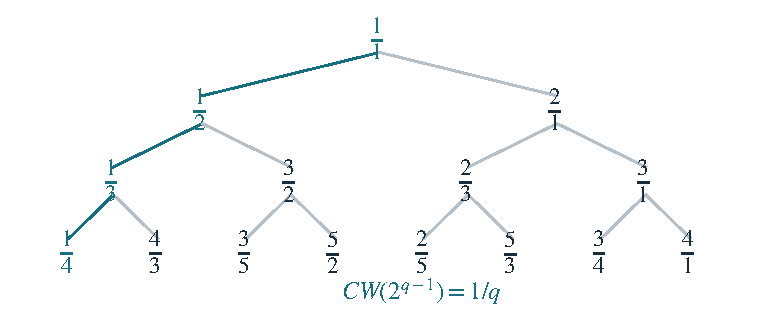
\includegraphics[width=.94\linewidth]{figuras/artigo_1/01_calkin_wilf.pdf}
\caption{Primeiros níveis da árvore de Calkin--Wilf. O ramo esquerdo contém $1/q$ no índice $2^{q-1}$; a ordenação por altura fornece índices polinomiais na altura.}\label{artigo_1:fig:cw}\end{figure}
% FIM artigos/artigo_1/secoes/02_indexacao.tex
% INICIO artigos/artigo_1/secoes/03_biblioteca.tex
\section{Células diádicas e operador gerador}
\subsection{Células, posse e centros}
Para $k\in\N_0$ e $m\in\Z$, sejam
\eqn{09}{J_{k,m}=[m2^{-k},(m+1)2^{-k}],\qquad J_{k,m}^{\rm own}=[m2^{-k},(m+1)2^{-k}),}
e
\eqn{10}{x_0(k,m)=\left(m+\frac12\right)2^{-k}=\frac{2m+1}{2^{k+1}}.}
A célula fechada sustenta o segmento; a versão semiaberta atribui cada fronteira a um único proprietário. Escreva
\[
\D=\{j2^{-K}:j\in\Z,\ K\in\N_0\},\qquad \D_{\rm mid}=\D\setminus\Z.
\]
% MAPA artigo_1:3.1 | fonte artigos/artigo_1/secoes/03_biblioteca.tex:11
\begin{lema}[estrutura diádica]\label{map:artigo_1:3.1}
Para cada $k$, as células $J_{k,m}^{\rm own}$ particionam $\R$ e
\eqn{11}{J_{k,m}=J_{k+1,2m}\cup J_{k+1,2m+1},\qquad |J_{k,m}|=2^{-k}.}
O mapa $(k,m)\mapsto x_0(k,m)$ é uma bijeção de $\N_0\times\Z$ sobre $\D_{\rm mid}$, que é denso em $\R$.
\end{lema}
\begin{proof}
Para $x\in\R$, o único índice de posse na escala $k$ é $m=\lfloor2^kx\rfloor$; isso prova a partição. A identidade de refinamento decorre de cindir $[2m2^{-(k+1)},(2m+2)2^{-(k+1)}]$ em seu ponto médio.

Pela \eqref{artigo_1:eq:10}, o centro tem numerador ímpar e denominador reduzido $2^{k+1}\ge2$, logo pertence a $\D_{\rm mid}$. Reciprocamente, cada $x\in\D_{\rm mid}$ possui forma reduzida única $j/2^K$, com $K\ge1$ e $j$ ímpar; tomando $k=K-1$ e $m=(j-1)/2$, obtém-se $x=x_0(k,m)$. A mesma unicidade prova a injetividade. Por fim, os centros de escala $k$ estão espaçados por $2^{-k}$; escolhendo o mais próximo de um real dado, a distância tende a zero com $k$, o que prova a densidade.
\end{proof}
\begin{figure}[!htbp]\centering
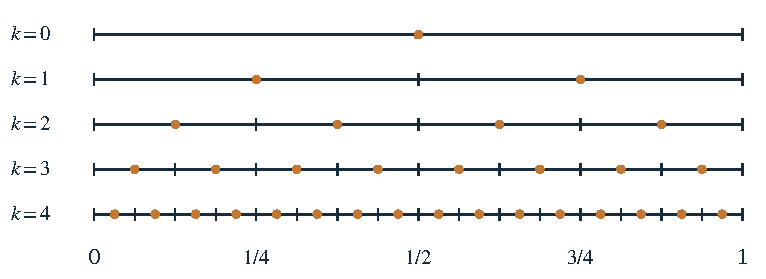
\includegraphics[width=.92\linewidth]{figuras/artigo_1/02_celulas.pdf}
\caption{Células diádicas, centros e posse das fronteiras. Cada célula se divide em dois filhos; os centros determinam a célula de origem.}\label{artigo_1:fig:celulas}\end{figure}

\subsection{Retas ancoradas e descompactação}
Dados $x_0,y_0\in\R$ e $s\ne0$, a reta ancorada é
\eqn{12}{\ell(x)=y_0+s(x-x_0)=a+bx,\qquad b=s,\quad a=y_0-sx_0.}
Para $n\in\N_0$, aplique sucessivamente a inversa do pareamento:
\eqn{13}{(u,v)=\pi^{-1}(n),\qquad(k,\mu)=\pi^{-1}(u),\qquad(r,t)=\pi^{-1}(v).}
% MAPA artigo_1:3.2 | fonte artigos/artigo_1/secoes/03_biblioteca.tex:28
\begin{lema}\label{map:artigo_1:3.2}
O mapa $n\mapsto(k,\mu,r,t)$ de \eqref{artigo_1:eq:13} é uma bijeção de $\N_0$ sobre $\N_0^4$.
\end{lema}
\begin{proof}
Sua inversa explícita é
\[
(k,\mu,r,t)\longmapsto\pi\bigl(\pi(k,\mu),\pi(r,t)\bigr),
\]
uma composição de bijeções pelo lema~2.1.
\end{proof}
Defina
\eqn{14}{m=Z(\mu),\quad x_{0,n}=x_0(k,m),\quad y_{0,n}=Q(r),\quad s_n=Q^*(t),}
e converta para a forma global por
\eqn{15}{b_n=s_n,\qquad a_n=y_{0,n}-s_nx_{0,n}.}
Se $x_L=m2^{-k}$ e $x_R=(m+1)2^{-k}$, ponha
\eqn{16}{c_n=\min\{\ell_n(x_L),\ell_n(x_R)\},\qquad d_n=\max\{\ell_n(x_L),\ell_n(x_R)\}.}
% MAPA artigo_1:3.3 | fonte artigos/artigo_1/secoes/03_biblioteca.tex:44
\begin{definicao}[gerador e biblioteca]\label{map:artigo_1:3.3}
Se $\mathcal I$ é o conjunto dos intervalos fechados não degenerados de $\R$, defina
\eqn{17}{\Gamma:\N_0\to\R\times(\R\setminus\{0\})\times\mathcal I,\qquad
\Gamma(n)=(a_n,b_n,[c_n,d_n]).}
A biblioteca é $\LL=\Gamma(\N_0)$. O átomo de endereço $n$ é a restrição de $\ell_n$ à célula $J_{k(n),m(n)}$.
\end{definicao}
Como $s_n\ne0$ e $x_L\ne x_R$, o intervalo em \eqref{artigo_1:eq:16} é não degenerado. A inclinação não nula torna a interface invertível no eixo espacial: uma peça constante teria imagem pontual e perderia a informação da célula. Para $\Gamma(n)=(a_n,b_n,[c_n,d_n])$, a pré-imagem espacial é
\eqn{18}{I_n^x=\left[
\min\left\{\frac{c_n-a_n}{b_n},\frac{d_n-a_n}{b_n}\right\},
\max\left\{\frac{c_n-a_n}{b_n},\frac{d_n-a_n}{b_n}\right\}\right].}

\subsection{Recuperação da célula e endereço canônico}
% MAPA artigo_1:3.4 | fonte artigos/artigo_1/secoes/03_biblioteca.tex:56
\begin{lema}[validade espacial exata]\label{map:artigo_1:3.4}
Para todo $n\in\N_0$, o intervalo $I_n^x$ definido em \eqref{artigo_1:eq:18} satisfaz
\[
I_n^x=J_{k(n),m(n)}.
\]
\end{lema}
\begin{proof}
Como $b_n\ne0$, $\ell_n$ é uma bijeção afim estritamente monótona. Sua restrição a $[x_L,x_R]$ tem imagem $[c_n,d_n]$ por \eqref{artigo_1:eq:16}; logo $\ell_n^{-1}([c_n,d_n])=[x_L,x_R]$. Os dois quocientes em \eqref{artigo_1:eq:18} são precisamente $\ell_n^{-1}(c_n)$ e $\ell_n^{-1}(d_n)$, possivelmente em ordem invertida quando $b_n<0$.
\end{proof}
% MAPA artigo_1:3.5 | fonte artigos/artigo_1/secoes/03_biblioteca.tex:65
\begin{teorema}[unicidade do endereço]\label{map:artigo_1:3.5}
$\Gamma$ é injetiva. Portanto, é uma bijeção de $\N_0$ sobre $\LL$ e cada átomo tem um único endereço.
\end{teorema}
\begin{proof}
Suponha $\Gamma(n)=\Gamma(n')=(a,b,[c,d])$. Pelo lema~3.4, a tripla recupera a célula comum $J=[x_L,x_R]$. Seu comprimento determina unicamente $k=-\log_2|J|$, e $m=2^kx_L$. Assim, também se recupera $x_0=(m+1/2)2^{-k}$. A inclinação local é $s=b$ e o valor ancorado é $y_0=a+bx_0$.

Pelas bijeções dos lemas~2.2, 2.4 e 3.1, os dados $(x_0,y_0,s)$ determinam unicamente $(k,\mu,r,t)$. O lema~3.2 determina então um único $n$. Logo $n=n'$.
\end{proof}
Em uma fronteira, duas células fechadas podem estar ativas. A célula semiaberta escolhe uma proprietária; em uma montagem contínua, as duas peças têm o mesmo valor no nó.
% MAPA artigo_1:3.6 | fonte artigos/artigo_1/secoes/03_biblioteca.tex:74
\begin{teorema}[dicionário de jatos racionais]\label{map:artigo_1:3.6}
O mapa
\eqn{19}{n\longmapsto(x_{0,n},y_{0,n},s_n)}
é uma bijeção de $\N_0$ sobre $\D_{\rm mid}\times\Q\times\Q^*$. Sua imagem é densa em $\R^3$.
\end{teorema}
\begin{proof}
A bijetividade resulta da composição das bijeções em \eqref{artigo_1:eq:13}--\eqref{artigo_1:eq:14}. A densidade decorre da densidade de $\D_{\rm mid}$, de $\Q$ e de $\Q^*$ em $\R$, aplicada coordenada a coordenada na norma do máximo.
\end{proof}
O dicionário \eqref{artigo_1:eq:19} parametriza todos os 1-jatos com centro diádico não inteiro, valor racional e derivada racional não nula. Montagens contínuas ligam esses dados locais por valores de fronteira compartilhados.

\subsection{Calibre dos parâmetros}
Para um átomo com dados $(k,m,y_0,s)$, usamos o mesmo calibre aritmético do segundo artigo:
\eqn{46}{H=\max\{2,k+1,|m|+1,\heightq(y_0),\heightq(s)\}.}
A definição fixa o significado da hipótese de altura na proposição~4.4; as contagens sob esse calibre são tratadas no segundo artigo.
% FIM artigos/artigo_1/secoes/03_biblioteca.tex
% INICIO artigos/artigo_1/secoes/04_montagens.tex
\section{Montagens e densidade em espaços de funções contínuas}
% MAPA artigo_1:4.1 | fonte artigos/artigo_1/secoes/04_montagens.tex:2
\begin{definicao}[montagem contínua]\label{map:artigo_1:4.1}
Se $K=[\alpha,\beta]$ é um intervalo compacto não degenerado, $\Asm(K)$ é o conjunto das funções $g\in C(K)$ para as quais existe uma coleção finita $\Lambda$ de células diádicas, com interiores disjuntos e união contendo $K$, e endereços $n(J)$, $J\in\Lambda$, tais que
\eqn{20}{g|_{J\cap K}=\ell_{n(J)}|_{J\cap K},}
com valores coincidentes nas fronteiras compartilhadas.
\end{definicao}
Para $f\in C(K)$, denote o módulo de continuidade por
\eqn{21}{\omega(f;\delta)=\sup\{|f(x)-f(y)|:x,y\in K,\ |x-y|\le\delta\}.}
O resultado seguinte impõe simultaneamente nós diádicos, valores racionais e inclinações não nulas. A figura~\ref{artigo_1:fig:montagem} mostra a ligação das peças por nós comuns.
\begin{figure}[!htbp]\centering
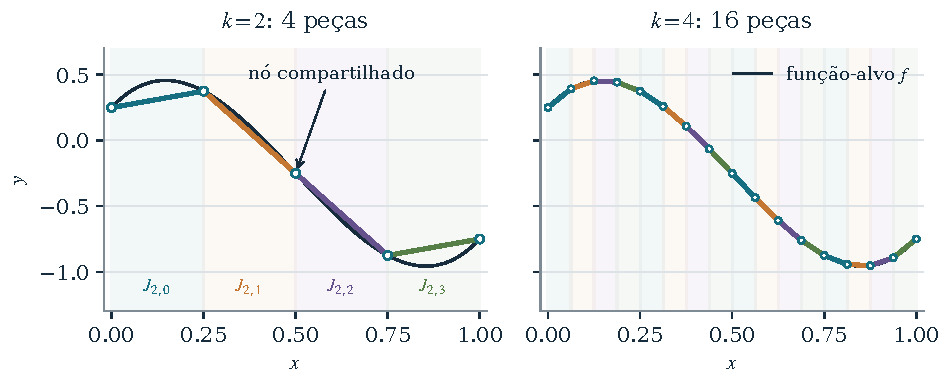
\includegraphics[width=1\linewidth]{figuras/artigo_1/03_montagem_continua.pdf}
\caption{Montagem contínua de átomos. À esquerda, cada cor identifica uma célula e seu segmento; peças consecutivas compartilham o mesmo valor no nó. À direita, o refinamento substitui células por filhos e aproxima a função-alvo com mais peças conectadas.}\label{artigo_1:fig:montagem}\end{figure}

% MAPA artigo_1:4.2 | fonte artigos/artigo_1/secoes/04_montagens.tex:12
\begin{teorema}[densidade das montagens]\label{map:artigo_1:4.2}
Para todo $f\in C[\alpha,\beta]$ e todo $\varepsilon>0$, existe $g\in\Asm([\alpha,\beta])$ tal que
\[
\normK{f-g}{[\alpha,\beta]}<\varepsilon.
\]
Todas as peças de $g$ pertencem a $\LL$ e têm inclinação não nula.
\end{teorema}
\begin{proof}
Estenda $f$ por constantes: $F(x)=f(\alpha)$ para $x<\alpha$, $F=f$ em $[\alpha,\beta]$ e $F(x)=f(\beta)$ para $x>\beta$. A extensão é uniformemente contínua. Escolha $k$ de modo que, com $h=2^{-k}$,
\eqn{22}{\omega(F;h)<\varepsilon/2.}
Tome os nós $t_j=jh$ desde $j_{\min}=\lfloor\alpha/h\rfloor$ até $j_{\max}=\lceil\beta/h\rceil$. Para cada $j$, escolha racional $v_j$ com $|v_j-F(t_j)|<\varepsilon/2$ e, sequencialmente, imponha $v_{j+1}\ne v_j$. Isso é possível porque cada intervalo aberto de escolha contém infinitos racionais e apenas um valor é proibido em cada passo.

Seja $g$ o interpolante linear dos pares $(t_j,v_j)$. Em $J_{k,j}$, sua inclinação é $(v_{j+1}-v_j)/h\in\Q^*$ e seu valor no centro é $(v_j+v_{j+1})/2\in\Q$. Pelo teorema~3.6, a peça é o único átomo com esses parâmetros. Os valores nodais compartilhados tornam $g$ contínua.

Se $P_kF$ é o interpolante dos valores exatos, então, para $x=(1-\theta)t_j+\theta t_{j+1}$,
\[
|F(x)-P_kF(x)|\le(1-\theta)|F(x)-F(t_j)|+\theta|F(x)-F(t_{j+1})|
\le\omega(F;h)<\varepsilon/2.
\]
Além disso, $P_kF-g$ é linear em cada célula e seus valores nodais têm módulo menor que $\varepsilon/2$, logo $\norm{P_kF-g}<\varepsilon/2$. A desigualdade triangular conclui.
\end{proof}
O número de células dessa cobertura uniforme é
\eqn{23}{N_k=\lceil\beta2^k\rceil-\lfloor\alpha2^k\rfloor=(\beta-\alpha)2^k+O(1).}

\subsection{Equivalência exata com redes ReLU racionais}
Escreva $\rho(z)=z_+=\max\{0,z\}$. A identidade em hinges abaixo conserva os nós diádicos, os parâmetros racionais e as inclinações não nulas da montagem.
% MAPA artigo_1:4.3 | fonte artigos/artigo_1/secoes/04_montagens.tex:38
\begin{teorema}[equivalência montagem--ReLU racional]\label{map:artigo_1:4.3}
Seja $g\in\Asm(K)$ dada por $N$ folhas consecutivas, com nós $t_0<t_1<\cdots<t_N$ e inclinação racional não nula $s_j$ em $[t_j,t_{j+1}]\cap K$, $0\le j<N$. Como $t_0$ pode estar fora de $K$, $g(t_0)$ denota o valor em $t_0$ da primeira peça $\ell_{n(J_0)}$, $J_0=[t_0,t_1]$, que coincide com $g(t_0)$ quando $t_0\in K$. Então, em $K$,
\eqn{24}{g(x)=g(t_0)+s_0(x-t_0)+\sum_{j=1}^{N-1}(s_j-s_{j-1})\rho(x-t_j).}
Depois de expandido o primeiro termo afim, todos os coeficientes são racionais, todos os pontos de quebra internos são diádicos e \eqref{artigo_1:eq:24} é uma rede ReLU rasa normalizada com $N-1$ unidades hinge e um termo afim de saída. Unidades cujo peso de saída é zero podem ser removidas.

Reciprocamente, seja
\eqn{25}{R(x)=c+qx+\sum_{j=1}^Ma_j\rho(x-\tau_j),\qquad c,q,a_j\in\Q,\quad\tau_j\in\D,}
com nós distintos. Suponha que $K$ admita uma cobertura por células diádicas compatível com os $\tau_j$, que os valores nodais sejam racionais e que cada inclinação local
\eqn{26}{q+\sum_{\tau_j<x}a_j}
seja não nula. Então $R|_K\in\Asm(K)$. Uma malha diádica uniforme que refine todos os $\tau_j$ fornece essa montagem explicitamente.
\end{teorema}
\begin{proof}
Na primeira folha, o lado direito de \eqref{artigo_1:eq:24} tem valor $g(t_0)$ em $t_0$ e inclinação $s_0$. Ao atravessar $t_j$, a derivada ganha exatamente $s_j-s_{j-1}$; por indução, sua inclinação na folha $j$ é $s_j$. Como ambos os lados são contínuos e coincidem no primeiro nó, coincidem em todo $K$. Cada $s_j$ é racional. Os nós internos são fronteiras de células diádicas, e o intercepto do primeiro átomo é racional por \eqref{artigo_1:eq:15}; logo a forma expandida tem somente parâmetros racionais.

Para a recíproca, refine uma grade diádica até que cada $\tau_j$ seja uma fronteira. Em qualquer célula aberta da grade, \eqref{artigo_1:eq:25} é afim, com inclinação \eqref{artigo_1:eq:26}. O valor no centro da célula é racional, pois o centro, os nós e todos os coeficientes são racionais. A hipótese de inclinação não nula permite aplicar o teorema~3.6, que fornece um único átomo da biblioteca nessa célula. A continuidade de $R$ faz os valores coincidirem nas fronteiras. A união das peças é, portanto, uma montagem no sentido da definição~4.1.
\end{proof}
A forma normalizada \eqref{artigo_1:eq:25} já implica valores nodais racionais. Se a arquitetura não oferecer conexão afim direta, $x=\rho(x)-\rho(-x)$ realiza o termo linear com duas unidades adicionais e viés constante na saída.

% MAPA artigo_1:4.4 | fonte artigos/artigo_1/secoes/04_montagens.tex:56
\begin{proposicao}[parâmetros e altura]\label{map:artigo_1:4.4}
Na forma normalizada, a conversão de uma montagem com $N$ folhas armazena $2N$ racionais: o intercepto e a inclinação iniciais, mais um nó e um salto de inclinação para cada uma das $N-1$ unidades. Se todos os átomos têm altura no máximo $H\ge2$, a altura máxima dos parâmetros produzidos satisfaz
\eqn{27}{H_{\rm ReLU}\le2^{H+1}H^2.}
\end{proposicao}
\begin{proof}
Há $N-1$ pares $(t_j,s_j-s_{j-1})$, além dos dois parâmetros afins. Pela definição de altura atômica, $\heightq(s_j)\le H$, os nós satisfazem $\heightq(t_j)\le2^H$, e a forma geral do \cref{artigo_2:lem:height-arithmetic} dá $\heightq(s_j-s_{j-1})\le2H^2$. Para o intercepto inicial, escreva $a=y_0-sx_0$. Como $\heightq(x_0)\le2^H$,
\[
\heightq(a)\le2\heightq(y_0)\heightq(sx_0)\le2^{H+1}H^2.
\]
Isso prova \eqref{artigo_1:eq:27}. Como os demais parâmetros são produtos ou somas dos mesmos dados, essa cota também garante que a conversão é efetiva em aritmética racional exata.
\end{proof}
\begin{figure}[!htbp]\centering
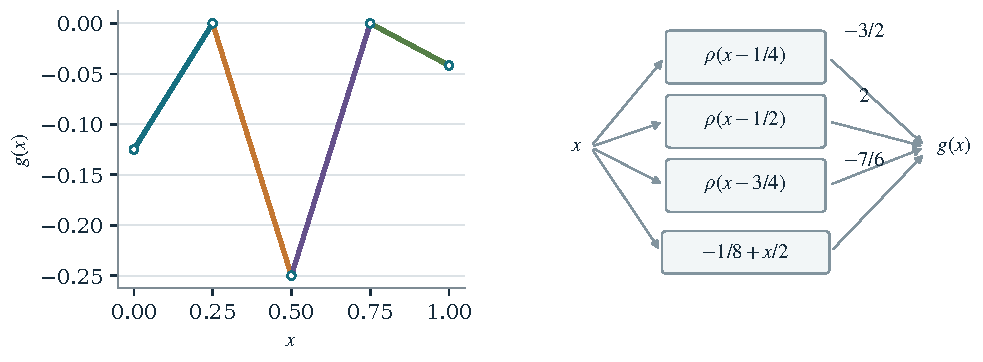
\includegraphics[width=1\linewidth]{figuras/artigo_1/04_relu.pdf}
\caption{Uma montagem racional com quatro folhas e a rede ReLU rasa dada pela identidade \eqref{artigo_1:eq:24}. O gráfico e os pesos são calculados a partir dos mesmos dados racionais.}\label{artigo_1:fig:relu}\end{figure}
A identidade funcional do teorema~4.3 conduz aos formatos da \cref{artigo_2:subsec:coding-formats}, que distinguem a transmissão estrutural dos diádicos de sua expansão em frações reduzidas.

\subsection{Relação com o 1-jato de Taylor}
Se $J_{k,m}$ tem centro $x_0$ e largura $h$, o 1-jato de $f\in C^2(J_{k,m})$ é
\[
T_{x_0}f(x)=f(x_0)+f'(x_0)(x-x_0).
\]
% MAPA artigo_1:4.5 | fonte artigos/artigo_1/secoes/04_montagens.tex:75
\begin{proposicao}[pertencimento e aderência]\label{map:artigo_1:4.5}
Se $f(x_0)\in\Q$ e $f'(x_0)\in\Q^*$, então $T_{x_0}f$ é o átomo de $\LL$ associado à célula. Em geral, para todo $\delta>0$ existem $q_0\in\Q$ e $q_1\in\Q^*$ tais que $\ell_q(x)=q_0+q_1(x-x_0)$ satisfaz
\eqn{28}{\normK{T_{x_0}f-\ell_q}{J_{k,m}}<\delta,}
\eqn{29}{\normK{f-\ell_q}{J_{k,m}}\le\frac{h^2}8\normK{f''}{J_{k,m}}+\delta.}
\end{proposicao}
\begin{proof}
No primeiro caso, $(x_0,f(x_0),f'(x_0))$ pertence ao contradomínio do teorema~3.6. No caso geral, escolha $q_0$ com $|f(x_0)-q_0|<\delta/2$ e $q_1\ne0$ com $|f'(x_0)-q_1|<\delta/h$. Como $|x-x_0|\le h/2$, obtém-se \eqref{artigo_1:eq:28}. O resto integral de Taylor fornece
\[
|f(x)-T_{x_0}f(x)|=\left|\int_{x_0}^x(x-t)f''(t)\,dt\right|
\le\frac{|x-x_0|^2}2\norm{f''}\le\frac{h^2}8\norm{f''}.
\]
A desigualdade triangular prova \eqref{artigo_1:eq:29}.
\end{proof}
Jatos reais arbitrários pertencem, portanto, à aderência local da biblioteca racional.
% FIM artigos/artigo_1/secoes/04_montagens.tex
% INICIO artigos/artigo_1/secoes/05_taxas.tex
\section{Taxas uniformes e constante assintótica}
Para $f\in C^2[\alpha,\beta]$, use a extensão
\eqn{30}{F(x)=\begin{cases}
f(\alpha)+f'(\alpha)(x-\alpha)+\frac12f''(\alpha)(x-\alpha)^2,&x<\alpha,\\
f(x),&\alpha\le x\le\beta,\\
f(\beta)+f'(\beta)(x-\beta)+\frac12f''(\beta)(x-\beta)^2,&x>\beta.
\end{cases}}
Então $F\in C^2(\R)$ e $\normK{F''}{\R}=\normK{f''}{[\alpha,\beta]}$. Seja $P_kF$ o interpolante nos nós $j2^{-k}$.

% MAPA artigo_1:5.1 | fonte artigos/artigo_1/secoes/05_taxas.tex:10
\begin{teorema}[cota aguda e limite]\label{map:artigo_1:5.1}
Ponha $h=2^{-k}$ e $M=\normK{f''}{[\alpha,\beta]}$. Então
\eqn{31}{\normK{f-P_kF}{[\alpha,\beta]}\le\frac{h^2M}8,}
e
\eqn{32}{\lim_{k\to\infty}\frac8{h^2}\normK{f-P_kF}{[\alpha,\beta]}=M.}
Além disso, para todo $\delta>0$ existe $g_{k,\delta}\in\Asm([\alpha,\beta])$ com
\eqn{33}{\norm{f-g_{k,\delta}}\le\frac{h^2M}8+\delta.}
\end{teorema}
\begin{proof}
Em uma célula $[x_L,x_R]$ de largura $h$, ponha $e=F-P_kF$. Para $x\in(x_L,x_R)$, a função
\[
\psi(t)=e(t)-\frac{(t-x_L)(t-x_R)}{(x-x_L)(x-x_R)}e(x)
\]
anula-se em $x_L,x,x_R$. Três aplicações de Rolle produzem $\xi_x\in(x_L,x_R)$ com $\psi''(\xi_x)=0$; portanto
\eqn{34}{F(x)-P_kF(x)=\frac12F''(\xi_x)(x-x_L)(x-x_R).}
O módulo do produto é no máximo $h^2/4$, com igualdade no centro, o que prova \eqref{artigo_1:eq:31}.

Se $M=0$, \eqref{artigo_1:eq:32} é imediata. Se $M>0$, escolha $x_*\in[\alpha,\beta]$ com $|f''(x_*)|=M$. Para cada $k$ suficientemente grande, escolha um centro de escala $k$, $z_k\in[\alpha,\beta]$, com $z_k\to x_*$. Avaliando \eqref{artigo_1:eq:34} em $z_k$,
\[
|F(z_k)-P_kF(z_k)|=\frac{h^2}8|F''(\xi_k)|,
\]
onde $\xi_k$ pertence à célula de $z_k$. O diâmetro da célula tende a zero, logo $\xi_k\to x_*$ e $|F''(\xi_k)|\to M$. Isso dá o limite inferior; \eqref{artigo_1:eq:31} fornece o superior.

Para a última afirmação, racionalize todos os valores nodais da cobertura finita com erro menor que $\delta$ e mantenha valores adjacentes distintos, como no teorema~4.2. O interpolante resultante é uma montagem e dista menos que $\delta$ de $P_kF$ em norma uniforme. A desigualdade triangular conclui.
\end{proof}

% MAPA artigo_1:5.2 | fonte artigos/artigo_1/secoes/05_taxas.tex:36
\begin{corolario}[preservação da constante]\label{map:artigo_1:5.2}
Existe uma sequência $g_k\in\Asm([\alpha,\beta])$ tal que
\[
\lim_{k\to\infty}\frac8{h^2}\norm{f-g_k}=M.
\]
\end{corolario}
\begin{proof}
Na construção do teorema~5.1, escolha erros nodais $\delta_k=o(h^2)$. Então
\[
\left|\norm{f-g_k}-\norm{f-P_kF}\right|\le\norm{g_k-P_kF}<\delta_k.
\]
Divida por $h^2/8$ e aplique \eqref{artigo_1:eq:32}.
\end{proof}
Com $N_k$ de \eqref{artigo_1:eq:23}, $h=(\beta-\alpha)N_k^{-1}(1+O(N_k^{-1}))$ e, portanto,
\eqn{35}{\norm{f-P_kF}\le\frac{(\beta-\alpha)^2M}8N_k^{-2}\bigl(1+O(N_k^{-1})\bigr).}
Quando os extremos já são nós da malha, o termo de borda desaparece.
\begin{table}[!htbp]\centering
\caption{Erro exato do interpolante de $e^x$ em $[0,1]$.}
\begin{tabular}{rrrr}\toprule
$k$&erro exato&$2^{-2k}e/8$&razão\\\midrule
2&$1{,}8774\times10^{-2}$&$2{,}1237\times10^{-2}$&$0{,}8840$\\
4&$1{,}2866\times10^{-3}$&$1{,}3273\times10^{-3}$&$0{,}9693$\\
6&$8{,}2310\times10^{-5}$&$8{,}2955\times10^{-5}$&$0{,}9922$\\
8&$5{,}1746\times10^{-6}$&$5{,}1847\times10^{-6}$&$0{,}9980$\\
10&$3{,}2389\times10^{-7}$&$3{,}2404\times10^{-7}$&$0{,}9995$\\\bottomrule
\end{tabular}
\end{table}
\begin{figure}[!htbp]\centering
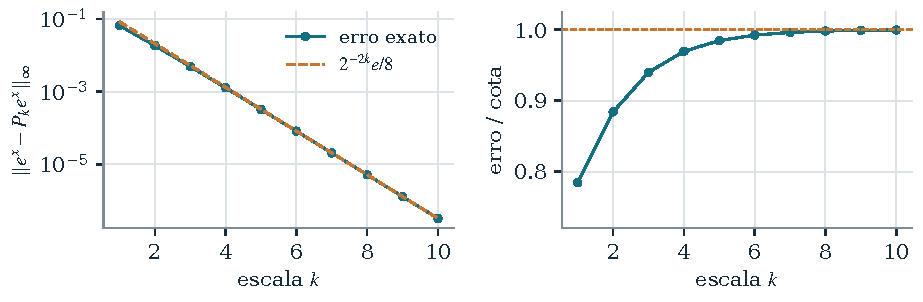
\includegraphics[width=.98\linewidth]{figuras/artigo_1/05_taxa_exponencial.pdf}
\caption{Erro do interpolante de $e^x$ e razão entre erro e cota. A razão converge a $1$, conforme \eqref{artigo_1:eq:32}.}\label{artigo_1:fig:taxa}\end{figure}
% FIM artigos/artigo_1/secoes/05_taxas.tex
% INICIO artigos/artigo_1/secoes/06_refinamento.tex
\section{Refinamento diádico adaptativo certificado}
O refinamento usa majorantes locais validados de $|F''|$ para controlar o erro em cada célula.

\subsection{Fechamento operacional por aritmética intervalar}
Seja $\EE$ a menor classe de expressões que contém $x$ e as constantes racionais e é fechada por soma, subtração, produto, recíproco, $\exp$, $\sin$, $\cos$ e composição. Um recíproco é admissível em intervalos nos quais seu denominador não se anula. Essa classe contém os polinômios, as funções racionais sem polos no domínio e as funções elementares usadas nos exemplos.

Composição significa substituição sintática: em $u\circ v$, cada folha $x$ da árvore de $u$ é substituída pela árvore de $v$. Toda expressão composta é, assim, uma árvore das operações-base.

Escreva $\mathbb I_{\Q}$ para os intervalos fechados com extremos racionais. A rotina
\eqn{36}{\operatorname{BoundSecondDerivative}(E,J;P,d)
=[\underline m_J,\overline m_J]\in\mathbb I_{\Q}}
usa precisão transcendental $P$ e profundidade de subdivisão $d$. Ela propaga simultaneamente intervalos para $(E,E',E'')$, isto é, 2-jatos intervalares. Por exemplo,
\begin{align*}
(uv)''&=u''v+2u'v'+uv'',\\
(u^{-1})''&=2(u')^2u^{-3}-u''u^{-2},\\
(e^u)''&=e^u\bigl((u')^2+u''\bigr),\\
(\sin u)''&=-\sin(u)(u')^2+\cos(u)u'',\\
(\cos u)''&=-\cos(u)(u')^2-\sin(u)u''.
\end{align*}
As operações racionais são exatas. Para $\exp$, a redução do argumento a $|z|\le1/2$ é seguida por uma soma de Taylor com resto majorado por uma série geométrica racional; para $\sin$ e $\cos$, usa-se o resto de Lagrange racional e a interseção com $[-1,1]$. Elevar $P$ e $d$ reduz a sobrestimação.

% MAPA artigo_1:6.1 | fonte artigos/artigo_1/secoes/06_refinamento.tex:22
\begin{lema}[restos transcendentais com extremos racionais]\label{map:artigo_1:6.1}
Se $I=[a,b]\in\mathbb I_{\Q}$, as rotinas descritas acima produzem intervalos de extremos racionais que contêm $\exp(I)$, $\sin(I)$ e $\cos(I)$. Mais explicitamente, para $0\le z\le1/2$ e $n\ge0$,
\eqn{37}{0\le e^z-\sum_{j=0}^n\frac{z^j}{j!}
\le\frac{z^{n+1}}{(n+1)!}\frac1{1-z/(n+2)}.}
Se $R=\max\{|a|,|b|\}$ e
\[
P_n^{\sin}(z)=\sum_{j=0}^n(-1)^j\frac{z^{2j+1}}{(2j+1)!},\qquad
P_n^{\cos}(z)=\sum_{j=0}^n(-1)^j\frac{z^{2j}}{(2j)!},
\]
então, para todo $z\in I$,
\eqn{38}{|\sin z-P_n^{\sin}(z)|\le\frac{R^{2n+2}}{(2n+2)!},\qquad
|\cos z-P_n^{\cos}(z)|\le\frac{R^{2n+1}}{(2n+1)!}.}
Avaliar os polinômios em $I$, inflar pelos respectivos restos e intersectar com $[-1,1]$ preserva a inclusão.
\end{lema}
\begin{proof}
Na série de $e^z$, o primeiro termo omitido é $t_{n+1}=z^{n+1}/(n+1)!$. Para $j\ge n+1$, a razão entre termos consecutivos é $z/(j+1)\le z/(n+2)<1$; a cauda é, portanto, majorada pela série geométrica de primeiro termo $t_{n+1}$ e razão $z/(n+2)$, o que dá \eqref{artigo_1:eq:37}. Para um argumento racional $x$ arbitrário, escolha $r$ com $z=|x|/2^r\le1/2$, aplique a inclusão anterior e eleve o intervalo ao quadrado $r$ vezes; se $x<0$, tome o recíproco do intervalo positivo obtido para $-x$. Em $I=[a,b]$, a monotonicidade de $e^x$ permite usar o extremo inferior da inclusão em $a$ e o superior da inclusão em $b$.

As duas desigualdades em \eqref{artigo_1:eq:38} são o resto de Lagrange dos polinômios de Maclaurin de graus $2n+1$ e $2n$, pois todas as derivadas de seno e cosseno têm módulo no máximo $1$. A avaliação intervalar contém a imagem de cada polinômio; inflar pelo raio do resto contém a função. Como seno e cosseno já pertencem a $[-1,1]$, a interseção não remove nenhum valor possível. Todas as operações, fatoriais e extremos envolvidos são racionais.
\end{proof}

% MAPA artigo_1:6.2 | fonte artigos/artigo_1/secoes/06_refinamento.tex:42
\begin{proposicao}[correção do majorante intervalar]\label{map:artigo_1:6.2}
Se $E\in\EE$ define uma função $C^2$ em $J$ e a rotina \eqref{artigo_1:eq:36} termina com sucesso, então
\eqn{39}{E''(x)\in[\underline m_J,\overline m_J]\ (x\in J),\qquad
M_{\rm int}(J):=\max\{|\underline m_J|,|\overline m_J|\}\ge\normK{E''}{J}.}
Se algum intervalo de denominador contém zero mesmo após a subdivisão permitida, a rotina devolve falha e nenhum número é aceito como certificado.
\end{proposicao}
\begin{proof}
Para constantes e para $x$, a inclusão é imediata. Soma, produto e recíproco preservam inclusão pelas operações elementares de intervalos; o recíproco só é executado quando zero está fora do intervalo do denominador. As fórmulas de 2-jatos acima e o lema~6.1 dão o passo de indução estrutural para toda expressão de $\EE$. Pela normalização sintática declarada antes do lema, uma composição genérica já foi expandida nessa árvore e não acrescenta um caso independente. Subdividir $J$ preserva a cobertura, e tomar o fecho convexo dos intervalos obtidos em suas partes contém a união das imagens de $E''$. Isso prova a primeira inclusão e, tomando módulos, \eqref{artigo_1:eq:39}. A regra de falha impede que uma divisão não validada produza uma falsa garantia.
\end{proof}
A propagação registra a largura dos intervalos, o número de caixas e a profundidade usados. Subdivisão e Taylor racional permitem apertar as inclusões.

% MAPA artigo_1:6.3 | fonte artigos/artigo_1/secoes/06_refinamento.tex:53
\begin{algoritmo}[refinamento certificado]\label{map:artigo_1:6.3}
Dados $f\in C^2[\alpha,\beta]$, tolerâncias $\varepsilon_I,\varepsilon_R>0$ e a extensão $F$ de \eqref{artigo_1:eq:30}, use, para toda célula $J$, um majorante validado
\eqn{40}{\normK{F''}{J}\le M(J)\le M_*<\infty.}
Quando $F$ é fornecida por uma expressão de $\EE$, tome $M(J)=M_{\rm int}(J)$ de \eqref{artigo_1:eq:39}; se a certificação falhar, aborte sem emitir uma montagem garantida. Para uma função $C^2$ fora dessa interface, \eqref{artigo_1:eq:40} é um contrato de entrada.
\begin{enumerate}[label=(\roman*),topsep=6pt,itemsep=3pt]
\item Inicie com uma cobertura diádica finita de $[\alpha,\beta]$.
\item Para cada folha $J$, calcule
\eqn{41}{\eta_{\rm cert}(J)=\frac{|J|^2M(J)}8.}
\item Enquanto existir folha com $\eta_{\rm cert}(J)>\varepsilon_I$, substitua-a por seus dois filhos.
\item Nos nós finais, escolha racionais compartilhados $v_t$ com $|v_t-F(t)|<\varepsilon_R$ e valores adjacentes distintos.
\item Emita, em cada folha, o endereço do átomo que interpola seus dois valores nodais.
\end{enumerate}
\end{algoritmo}

% MAPA artigo_1:6.4 | fonte artigos/artigo_1/secoes/06_refinamento.tex:67
\begin{teorema}[correção, término e tamanho]\label{map:artigo_1:6.4}
O algoritmo~6.3 termina e produz $g\in\Asm([\alpha,\beta])$ com
\eqn{42}{\norm{f-g}\le\varepsilon_I+\varepsilon_R.}
Se a cobertura inicial tem $R_0$ raízes de largura máxima $h_0$ e $M_*>0$, nenhuma ramificação ultrapassa
\eqn{43}{r_*=\max\left\{0,\left\lceil\frac12\log_2\left(\frac{h_0^2M_*}{8\varepsilon_I}\right)\right\rceil\right\}}
níveis, e há no máximo $R_02^{r_*}$ folhas. Se $M_*=0$, pode-se tomar $r_*=0$.
\end{teorema}
\begin{proof}
Após $r$ subdivisões, uma folha descendente de uma raiz tem $|J|\le h_02^{-r}$ e, por \eqref{artigo_1:eq:40},
\[
\eta_{\rm cert}(J)\le\frac{h_0^2M_*}8\,4^{-r}.
\]
O lado direito é no máximo $\varepsilon_I$ para $r\ge r_*$; logo nenhuma folha é subdividida além dessa profundidade. A árvore é finita e cada raiz gera no máximo $2^{r_*}$ folhas.

Na partição final, \eqref{artigo_1:eq:34} e \eqref{artigo_1:eq:40} implicam
\[
\normK{F-P_\Lambda F}{J}\le\frac{|J|^2}8\normK{F''}{J}\le\eta_{\rm cert}(J)\le\varepsilon_I.
\]
A racionalização nodal produz, pelos teoremas~3.5 e 3.6, uma montagem de átomos de endereço único e com $\norm{P_\Lambda F-g}<\varepsilon_R$. Como $F=f$ no intervalo original, a desigualdade triangular prova \eqref{artigo_1:eq:42}.
\end{proof}
\begin{figure}[H]\centering
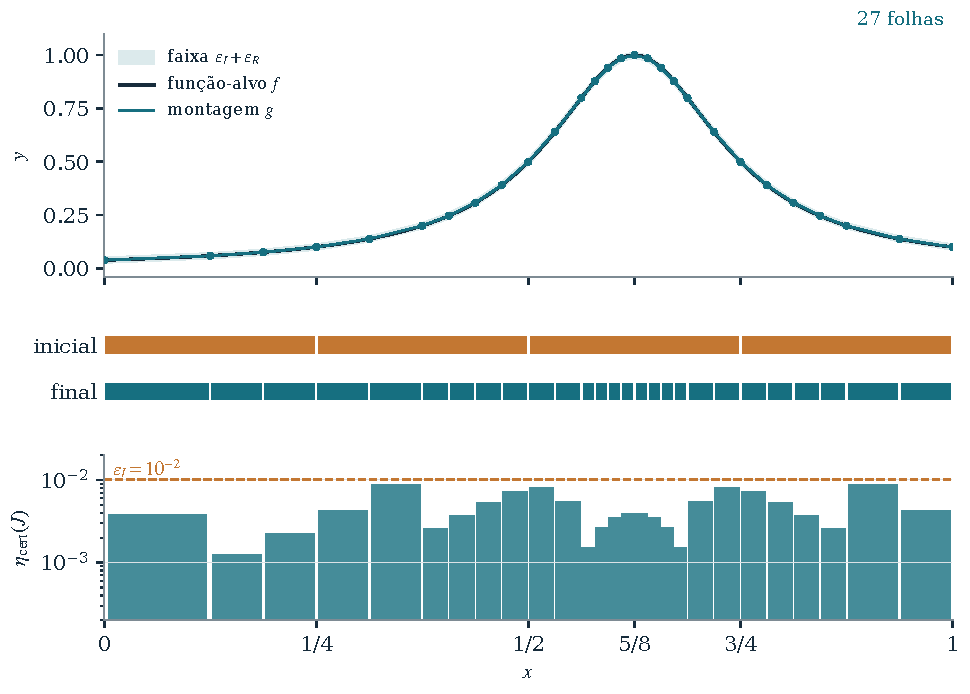
\includegraphics[width=.90\linewidth]{figuras/artigo_1/06_refinamento_certificado.pdf}
\caption{Refinamento certificado para $f(x)=[1+64(x-5/8)^2]^{-1}$. Células com certificado acima de $\varepsilon_I$ são subdivididas. A malha se concentra na região de maior curvatura, e o painel inferior compara os certificados finais com a tolerância. A faixa superior representa o limite uniforme $\varepsilon_I+\varepsilon_R$.}
\label{artigo_1:fig:refinamento}
\end{figure}

% MAPA artigo_1:6.5 | fonte artigos/artigo_1/secoes/06_refinamento.tex:93
\begin{proposicao}[calibração exata para curvatura constante]\label{map:artigo_1:6.5}
Suponha que $[\alpha,\beta]=J_0$ seja uma única célula diádica inicial, $F''\equiv\kappa\ne0$ em $J_0$ e $M(J)=|\kappa|$ em todo descendente. Pondo
\[
A=\frac{|J_0|^2|\kappa|}8,
\]
o número de folhas produzido com tolerância $\varepsilon_I$ é
\eqn{44}{N(\varepsilon_I)=2^{r(\varepsilon_I)},\qquad
r(\varepsilon_I)=\max\left\{0,\left\lceil\log_4\left(\frac A{\varepsilon_I}\right)\right\rceil\right\}.}
Consequentemente,
\eqn{45}{\begin{aligned}
\liminf_{\varepsilon_I\downarrow0}\sqrt{\varepsilon_I}\,N(\varepsilon_I)
&=\frac1{\sqrt8}\int_\alpha^\beta|f''(x)|^{1/2}\,dx,\\
\limsup_{\varepsilon_I\downarrow0}\sqrt{\varepsilon_I}\,N(\varepsilon_I)
&=\frac1{\sqrt2}\int_\alpha^\beta|f''(x)|^{1/2}\,dx.
\end{aligned}}
A quantização diádica introduz, nesse caso, um fator dois entre os limites de acumulação.
\end{proposicao}
\begin{proof}
Após $r$ subdivisões uniformes, cada folha tem largura $|J_0|2^{-r}$ e certificado $A4^{-r}$. Como todos os certificados de um mesmo nível são iguais, o algoritmo para no primeiro $r$ com $A4^{-r}\le\varepsilon_I$, o que prova \eqref{artigo_1:eq:44}. Para $A4^{-r}\le\varepsilon_I<A4^{-(r-1)}$, tem-se
\[
\sqrt A\le\sqrt{\varepsilon_I}\,2^r<2\sqrt A.
\]
Os extremos inferior e superior são atingidos, respectivamente, nos limiares $\varepsilon_I=A4^{-r}$ e por aproximação pela esquerda aos limiares $A4^{-(r-1)}$. Por fim, $\int_\alpha^\beta|f''|^{1/2}=|J_0|\sqrt{|\kappa|}$.
\end{proof}

% MAPA artigo_1:6.6 | fonte artigos/artigo_1/secoes/06_refinamento.tex:118
\begin{observacao}[diferença segunda e erro no centro]\label{map:artigo_1:6.6}
Se $x_0=(x_L+x_R)/2$, então
\[
|f(x_0)-P_Jf(x_0)|=\frac12|f(x_L)-2f(x_0)+f(x_R)|.
\]
Isso mede o erro no centro. Para $f(x)=x^3$ em $[-1,1]$, $P_Jf(x)=x$ e a diferença segunda central é zero, enquanto
\[
\norm{x^3-x}=\frac2{3\sqrt3}\approx0{,}3849.
\]
O controle em todo o intervalo é fornecido pelo majorante de \eqref{artigo_1:eq:40}.
\end{observacao}
% FIM artigos/artigo_1/secoes/06_refinamento.tex
% INICIO artigos/artigo_1/secoes/08_conclusao.tex
\begin{figure}[!htbp]
\centering
\begin{tikzpicture}[
 >=Latex,
 box/.style={draw=ink!65,rounded corners=2pt,fill=ink!3,
  align=center,text width=6.0cm,minimum height=.95cm,inner sep=5pt,font=\small},
 side/.style={box,text width=3.4cm},
 arr/.style={->,line width=.7pt,draw=ink!80},
 lab/.style={font=\footnotesize,fill=white,inner sep=1pt}]
\node[box] (in) {Entrada: $f$, domínio $K$, $\varepsilon_I,\varepsilon_R$\\expressão ou majorantes validados};
\node[box,below=4mm of in] (bound) {Cobertura diádica e aritmética intervalar\\$M(J)\ge\|F''\|_{\infty,J}$};
\node[box,below=4mm of bound,fill=accent!8,draw=accent] (test)
 {Teste local em cada folha\\$\eta_{\rm cert}(J)=|J|^2M(J)/8\le\varepsilon_I$};
\node[side,left=10mm of test] (split) {Subdividir $J$\\em dois filhos};
\node[box,below=7mm of test] (rational) {Nós racionais compartilhados\\$|v_t-F(t)|<\varepsilon_R$\\valores adjacentes distintos};
\node[box,below=4mm of rational] (atoms) {Montagem de átomos de $\LL$\\$\Gamma:\ n\leftrightarrow(k,m,y_0,s)\leftrightarrow(a,b,[c,d])$};
\node[side,anchor=north] (codec) at ($(atoms.south)+(-3.5,-.7)$)
 {Codificação\\$\Gamma^\sharp$ ou formatos\\atômico e ReLU};
\node[side,anchor=north] (catalog) at ($(atoms.south)+(3.5,-.7)$)
 {Truncagem $(D,H)$\\catálogo finito\\$\Sigma^{\LL}_{D,H}(K)$};
\node[side,below=4mm of codec,fill=accent!8] (out)
 {Decodificação exata de $g$\\$\|f-g\|_\infty\le\varepsilon_I+\varepsilon_R$};
\node[side,below=4mm of catalog,fill=accent!8] (min)
 {Mínimo de $\mathcal J$\\Desempate shortlex\\Representação canônica};
\draw[arr] (in)--(bound);
\draw[arr] (bound)--(test);
\draw[arr] (test.west)--node[lab,above]{não}(split.east);
\draw[arr] (split.north)|-(bound.west);
\draw[arr] (test)--node[lab,right]{sim, em todas as folhas}(rational);
\draw[arr] (rational)--(atoms);
\draw[arr] (atoms.south)--++(0,-.35)-|(codec.north);
\draw[arr] (atoms.south)--++(0,-.35)-|(catalog.north);
\draw[arr] (codec)--(out);
\draw[arr] (catalog)--(min);
\end{tikzpicture}
\caption{Circuito da construção: certificação local, refinamento, racionalização, endereçamento e descrição. A truncagem fornece a via finita de enumeração e minimização.}
\label{artigo_1:fig:circuito}
\end{figure}

\section{Conclusão}
A biblioteca $\LL$ reúne segmentos afins racionais com endereço único e suporte diádico recuperável. A bijeção com jatos racionais produz montagens contínuas densas em $C(K)$ e uma representação ReLU rasa exata. Na aproximação uniforme de funções $C^2$, a racionalização preserva a constante $1/8$ do erro interpolatório.

O refinamento adaptativo combina majorantes intervalares da segunda derivada e racionalização nodal para obter erro até $\varepsilon_I+\varepsilon_R$, com término e número de folhas controlados sob as hipóteses declaradas. A contagem aritmética, a codificação e a seleção exata são desenvolvidas no segundo artigo; as agendas de altura e a teoria direta--inversa, no terceiro. Os quatro resultados de referência não reproduzidos nesses recortes têm texto e demonstração preservados no complemento do original.
% FIM artigos/artigo_1/secoes/08_conclusao.tex
\clearpage
\section*{Apêndice da Parte I}\addcontentsline{toc}{section}{Apêndice da Parte I}
\setcounter{section}{0}\renewcommand{\thesection}{I.\Alph{section}}
% INICIO artigos/artigo_1/secoes/A_notacao.tex
\section{Quadro de notação}
\footnotesize
\renewcommand{\arraystretch}{1.1}
\begin{longtable}{@{}p{.28\linewidth}p{.68\linewidth}@{}}
\toprule Símbolo&Significado\\\midrule
\endfirsthead
\toprule Símbolo&Significado\\\midrule
\endhead
\bottomrule\endfoot
$\pi,\pi^{-1}$&Pareamento de Cantor e sua inversa.\\
$Z,Q,Q^*$&Enumerações de $\Z$, $\Q$ e $\Q^*$.\\
$\heightq(p/q)$&Altura $\max\{|p|,q\}$ da fração reduzida.\\
$\Q_H$&Racionais de altura no máximo $H$.\\
$\D,\D_{\rm mid}$&Diádicos e diádicos não inteiros.\\
$J_{k,m},J_{k,m}^{\rm own}$&Célula fechada e célula semiaberta de posse.\\
$x_0,y_0,s$&Centro, valor ancorado e inclinação de um átomo.\\
$\Gamma,\LL,\LL_H$&Gerador aritmético, biblioteca e truncagem por altura.\\
$I_n^x$&Suporte espacial recuperado da interface global.\\
$\Asm(K)$&Montagens contínuas finitas no domínio $K$.\\
$\omega(f;\delta)$&Módulo de continuidade de $f$.\\
$\rho(z)=z_+$&Ativação ReLU.\\
$P_kF,P_Jf,P_\Lambda F$&Interpolantes na malha uniforme, em uma célula e em uma partição.\\
$\EE,\mathbb I_{\Q}$&Gramática de expressões e intervalos de extremos racionais.\\
$P,d$&Precisão transcendental e profundidade de subdivisão intervalar.\\
$M_{\rm int}(J),M(J)$&Majorantes validados de $\|F''\|_{\infty,J}$.\\
$\eta_{\rm cert}(J)$&Certificado local $|J|^2M(J)/8$.\\
$\varepsilon_I,\varepsilon_R$&Tolerâncias de interpolação e racionalização.\\
$H$&Calibre atômico definido em \eqref{artigo_1:eq:46}.\\
\end{longtable}
\normalsize
% FIM artigos/artigo_1/secoes/A_notacao.tex
